\subsection{First Experience}

\subsubsection{Simple UDP capture}

After setting Wireshark's filter to display UDP only, and visiting
\textit{www.utec.edu.pe}, the total UDP packet count was approximately 69. Most
of them were outgoing packets. Their protocols varied between DNS, MDNS, DHCP,
and QUIC.\@

\begin{figure}[htbp]
    \centering
    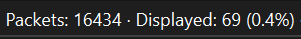
\includegraphics[width=1\linewidth]{img/1.png}
    \caption{Received UDP packet count}\label{fig:1}
\end{figure}

\begin{figure}[htbp]
    \centering
    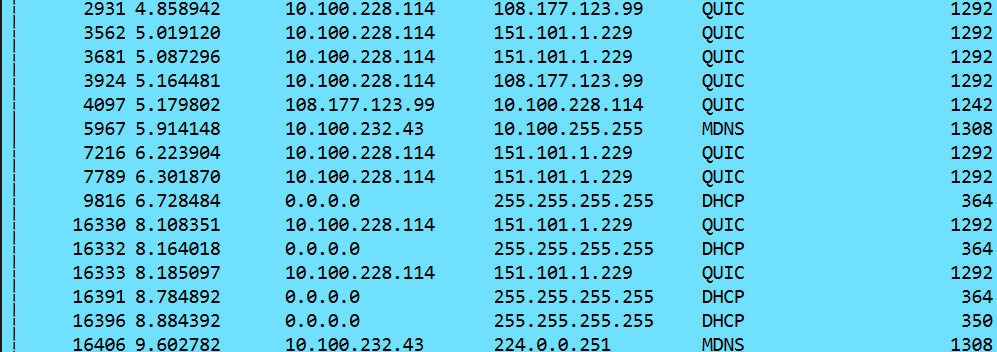
\includegraphics[width=1\linewidth]{img/2.png}
    \caption{UDP packet protocols}\label{fig:2}
\end{figure}

There were also many packets that were not necessarily related to the URL we
visited, such as a DNS query to \textit{watson.events.data.microsoft.com}. This
specific hostname is related to Windows telemetry.

\begin{figure}[htbp]
    \centering
    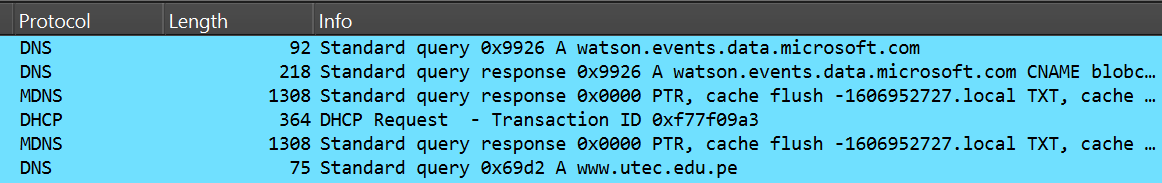
\includegraphics[width=1\linewidth]{img/3.png}
    \caption{Windows telemetry~\ensuremath{:(}}\label{fig:3}
\end{figure}

After that, we selected the first outgoing DNS packet going to
\textit{www.utec.edu.pe} to analyze its contents, which are displayed below.

\begin{figure}[htbp]
    \centering
    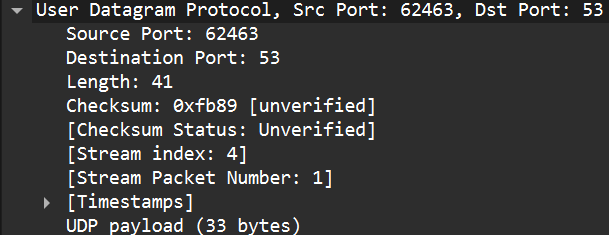
\includegraphics[width=1\linewidth]{img/4.png}
    \caption{www.utec.edu.pe packet info}\label{fig:4}
\end{figure}

The packet's main fields are:

\begin{itemize}
    \item Source/Destination Port: Port used for outgoing packet, destination port is the
          default DNS port (53).
    \item Length: Total length of the UDP packet (41 bytes).
    \item Checksum:
\end{itemize}

Test\cite{tanenbaum:networks}

\subsubsection{Using nslookup}

